\documentclass[12pt]{report}
\usepackage[utf8]{inputenc}
\usepackage{graphicx}
\usepackage{fancyhdr}



\title{ETERNITY: FUNCTION}
\author{Avneet Kaur Pannu}
\date{July 2022}

\makeatletter
\let\thetitle\@title
\let\theauthor\@author
\let\thedate\@date
\makeatother

\pagestyle{fancy}
\fancyhf{}
\rhead{\thetitle}
\cfoot{\thepage}

\begin{document}

\begin{titlepage}
	\centering
    \vspace*{0.5 cm}
\begin{center}    \textsc{\Large Concordia University}\\[2.0 cm]	\end{center}
	\textsc{\Large  SOEN 6011 - Software Engineering Process }\\[0.5 cm]
	\rule{\linewidth}{0.2 mm} \\[0.4 cm]
	{ \huge \textbf \thetitle}\\[0.2 cm]
	{ \huge \textbf{}}
	\rule{\linewidth}{0.2 mm} \\[1.5 cm]

\begin{center}   {\Large Deliverable 1}\\[2.0 cm]
	
\end{center}
	
\end{titlepage}

\renewcommand{\thesection}{\arabic{section}}
\tableofcontents
\pagebreak

\section{Introduction}
An exponential function is a function with the general form $ab^{x}$, $a\neq 0$, b is a positive real number and $b\neq 1$ .In an exponential function, a is constant, the base b is a constant, and the exponent x is a real variable.

\subsection{Domain}
\begin{itemize}
\item The domain is all Real numbers.
\\$- \infty < x < + \infty$, $x \in R$
\end{itemize}

\subsection{Co-Domain}
\begin{itemize}
  \item  $For$ $ b > 0$ , range is $[0,\infty)$  where $ b \in R$  and  $x \in R$. 
  \item  $For$ $ b = 0$ and $y =0$, range is 1 and  $For$ $ b = 0$ and $x>0$, range is 0.
 \item  $For$ $ b < 0$ , range is $(-\infty,\infty)$  where $ b \in R$  and  $x \in Z$.
\end{itemize}

\subsection{Characteristic}
\begin{itemize}


  \item \textbf{Exponential growth} : In the function  f(x) = $b^{x}$ when  $b > 1$, the function represents exponential growth. In figure 1, it is evident on the left side. 

  \item \textbf{Exponential decay} : In the function  f(x) = $b^{x}$ when  $0 < b < 1$, the function represents exponential decay. In figure 1, it is evident on the right side. 
  
   \item \textbf{Commutativity}:  Exponential function is not commutative which means $x^y \ne y^x $ for $x\ne y$. For example, $0^1 = 0$ and $1^0 = 1$.
   
\begin{figure}
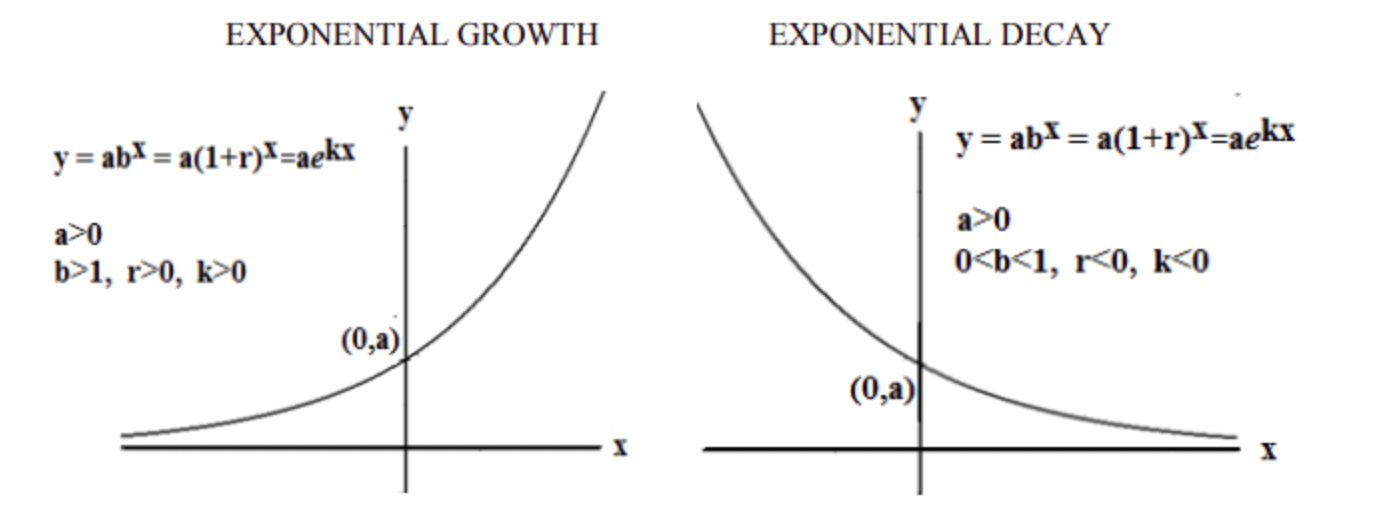
\includegraphics[width=15cm]{ExponentialGrowthandDecay.png}
\caption{Exponential Growth and Exponential Decay}
\label{exp}
\end{figure}



\end{itemize}

\section{Functional Requirement}
\subsection{Assumptions}
\subsection{Requirements}
\section{Algorithm}
\subsection{Description}
\subsection{Advantages and Disadvantages}



\end{document}
